% !TEX root = thesis.tex

%\section{Introduction}

\begin{abstract}

\end{abstract}
\tableofcontents
%\listoffigures

\clearpage
\section{Introduction}
{\color{red} REWRITE
 At sufficiently high energies quarks and gluons are no longer bound to hadrons, but they form a deconfined state known as Quark-Gluon plasma (QGP). The main goal of heavy-ion physics is the study of QGP and its properties.
One of the experimental observables that is sensitive to the properties of QGP is the azimuthal distribution of particles in the plane perpendicular to the beam direction. 

When nuclei collide at non-zero impact parameter (non-central collisions), their overlap region is asymmetric. This initial spatial asymmetry is converted via multiple collisions into an anisotropic momentum distribution of the produced particles. For low momentum particles ($\pt{} \lesssim 3$ \gevc), this anisotropy is understood to result from hydrodynamically driven flow of the QGP~\cite{Adcox:2004mh, Adams:2005dq, Ollitrault:1992, Heinz:2002, Shuryak:2009}. 

One way to characterize this anisotropy is with coefficients from a Fourier series parametrization of the azimuthal angle distribution of emitted hadrons. The second order coefficient, $v_2$ which is also known as elliptic flow, shows clear dependence on centrality. The collision geometry is mainly responsible for the elliptic flow. Higher harmonics don't depend that much on centrality. These higher harmonics carry information about the fluctuations in collisions. The event-by-event fluctuations have an increasing importance in measurements and it has been observed that measurements of elliptic flow in central collisions and measurements of higher order harmonics are consistent with the assumption that flow in these cases is mainly due to fluctuations~\cite{Jia:2012ve}.



At LHC energies  $\sqrt{s_{NN}}=2.76\mathrm{GeV}$ it has been observed that in general there is little difference to flow at RHIC energies. The $v_2$ coefficient is about 20\% greater at LHC than at RHIC, depending on the centrality bin. 
The particle identified $v_2$ for kaons and pions follows the same trend. However it was observed that for proton $v_2$ the quark number scaling does not work~\cite{Lacey:2012ma}. So far there is no agreement of why this scaling breaks down at LHC or why it works so well at RHIC energies.
}


\pagebreak
\subsection{Quantum chromodynamics}
\subsubsection{Foundation of QCD}
There are four known basic interactions in the universe: gravity, electromagnetic, weak and strong interactions. The standard model of particle physics includes three of these, excluding the gravitational interaction. The theory of strong interactions is known as Quantum Chromodynamics (QCD).

The development of QCD began after the introduction of new powerful particle accelerators that were capable of particle physics research in the 1950s. Before this particles were mainly discovered from cosmic rays. Positrons, neutrons and muons were discovered in the 1930s and charged pions were discovered in 1947~\cite{Occhialini:1987nr,Lattes:1947mx}. The neutral pion was discovered in 1950~\cite{Bjorklund:1950}.

The Lawrence Berkeley National Laboratory started the Bevalac accelerator in 1954, Super Proton Synchrotron (SPS) in CERN began operating in 1959 and the Alternating Gradient Synchrotron (AGS) at Brookhaven started in 1960. With an energy of \unit[33]{\gev} AGS was the most powerful accelerator of that time. By the beginning of 1960s several new particles had been discovered. These included antiprotons~\cite{Chamberlain:1955ns}, antineutrons~\cite{Cork:1957nu}, $\Delta$-particles and the six hyperons ($\Xi^0$\cite{Alvarez:1959zz}, $\Xi^-$~\cite{Armenteros:1952nt}, $\Sigma^{\pm}$~\cite{Bonetti1953}, $\Sigma^0$~\cite{Plano1957} and $\Lambda$~\cite{Fowler:1953qpk}).

Facing this avalanche of new particles, physicists started the search for symmetries within them. Already in 1932 Heisenberg~\cite{Heisenberg:1932} 
had proposed an isospin model to explain similarities between the proton and the neutron. In 1962 Gell-Mann and Ne'eman presented that particles sharing the same quantum numbers (spin, parity) could be organised using the symmetry of SU(3).~\cite{Gell-Mann:1962} Heisenberg's Isospin model followed the symmetry of SU(2). Using the SU(3) model known baryons and mesons could be presented as octets. This also lead to the discovery of the $\Omega^{-}$~\cite{Barnes:1964ga} particle since this was missing from the SU(3) decouplet that included heavier baryons. 

The most simple representation of SU(3) was a triplet. Inside this triplet particles would have electric charges $\nicefrac{2}{3}$ or $-\nicefrac{1}{3}$. However, these had not been detected. In 1964 Gell-Mann~\cite{Gell-Mann:1964} and Zweig~\cite{Zweig:1964jf} proposed that baryons and mesons would be bound states of these three hypothetical triplet particles that Gell-Mann called quarks. Zweig's nomenclature, aces, didn't live on. Now we know that these are the $u$, $d$ and $s$ quarks. However, this original quark model without colour was violating the Pauli exclusion principle. For example the $\Omega^{-}$ particle is comprised of three $s$ quarks, two of which would have exactly the same quantum states, since spin can only have two values. 


The idea of colour had already been presented by Greenberg in 1964~\cite{Greenberg:1964}. In 1971 Gell-Mann and Fritzsch presented their model~\cite{Fritzsch:1972jv}, which solved the antisymmetry problem. They added a colour quantum number to quarks, which separated quarks of the same species. In the new colour model the baryonic wave function became

\begin{equation}
\left( qqq\right)\rightarrow\left(q_rq_gq_b-q_gq_rq_b+q_bq_rq_g-q_rq_bq_g+q_gq_bq_r-q_bq_gq_r\right),
\end{equation}


%improve
\noindent The colour model was also supported by experimental evidence. The decay rate of a neutral pion with the addition of colours is

\begin{equation}
\Lambda\left(\pi^0\rightarrow\gamma \gamma\right) = \frac{\alpha^2}{2\pi}\frac{N_c^2}{3^2}\frac{m_\pi^3}{f_\pi^2}.
\end{equation} 

\noindent For $N_c=3$ this gives \unit[7.75]{eV} and the measured value is $(7.86\pm0.54)\,\mathrm{eV}$~\cite{Williams:1988sg}.

Another observable that combines the colour information also to the number of quark flavours is the Drell-Ratio $R$~\cite{Krolikowski:1974jx}

\begin{equation}
R=\frac{\sigma\left(e^++e^-\rightarrow\mathrm{hadrons}\right)}{\sigma\left(e^++e^-\rightarrow\mu^++\mu^-\right)}=N_c\sum_fQ_f^2.
\end{equation}

\noindent This ratio has the numerical value 2 when including the three light quarks $u$, $d$ and $s$. When the collision energy reaches the threshold of heavy quark ($c$ and $b$) production processes this increases to $\nicefrac{10}{3}$ (for $f=u,d,s,c$) and \nicefrac{11}{3} (for $f=u,d,s,c,b$). The energy threshold ($\sqrt{s}\approx350\gev$) of $t\bar t$ production, has not been reached so far by any $e^+e^-$ colliders.

%\cite{Glashow:1970gm} Introduction of lepton-quark symmetry by Glashow,Iliopoulos and Maiani, proposal of a fourth (charmed) quark.
%\\cite{Bacci:1974za} ADONE Discovery of charm quark and $J/\Psi$
%\cite{Aubert:1974js} BNL
%\cite{Augustin:1974xw} SLAC



The colour model explained why no free quarks had been observed as only colour neutral states are possible. The simplest ways of producing a colour neutral object are the combination of three quarks, and the combination of a quark-antiquark pair. These are known as baryons and mesons.

First experimental indication of the existence of quarks came in 1969 when a series of experiments at the Stanford Linear Accelerator Center (SLAC) revealed that protons and neutrons appeared to have some substructure~\cite{Bloom:1969kcm, Breidenbach:1969kd}. For this discovery they eventually received the Nobel Prize in Physics in 1990~\cite{Nobel1990}. Bjorken demonstrated that these results could be explained if protons and neutrons were composed of virtually noninteracting pointlike particles~\cite{Bjorken:1968dy,Bjorken:1969ja}. Feynman~\cite{Feynman:1969ej} interpreted these objects as real particles and suggested they would be the quarks of Gell-Mann's model. At the time, however, this seemed mysterious; if all strongly interacting particles, hadrons, were composed of quarks, then quarks should surely be strongly interacting themselves. Why would they appear to be almost free inside hadrons? This turned out to be a key clue in formulating the theory of strong interactions.~\cite{Krauss:2017} 

After the addition of colour the main ingredients of QCD had been established. The final quantum field theory of Quantum Chromodynamics formed quickly between 1972 and 1974. Main part of this was the work by Gross, Wilczek, Politzer and George for non-abelian gauge field theories~\cite{gross1973ultraviolet, politzer1973reliable, gross1973asymptotically, gross1974asymptotically, georgi1974electroproduction}. The work showed that quarks would indeed be asymptotically free in a non-abelian theory, which explained the results from SLAC. Gross, Wilczek and Politzer received the Nobel Prize in Physics for their work~\cite{Nobel2004}. The role of gluons as a colour octet was presented by Fritzsch, Gell-Mann and Leutwyler in 1973~\cite{fritzsch1973advantages}. The theory had now 8 massless gluons to mediate the strong interaction.

%Nobel1990 to Friedman, Kendall and Taylor for SLAC results
%Nobel1976 to Richter and Ting

The quark model was extended in 1974 when the discovery of the charm quark and the first charmed hadron, $J/\Psi$, was simultaneously published by teams from the SLAC~\cite{Augustin:1974xw}, from Brookhaven National Laboratory~\cite{Aubert:1974js} and from the ADONE collider in Frascati, Italy~\cite{Bacci:1974za}. In 1976 the Nobel Prize in Physics was awarded to Richter and Ting for the discovery of the charm quark~\cite{Nobel1976}. The existence of a fourth quark had already been speculated in 1964 by Bjorken and Glashow~\cite{Bjorken:1964gz}, but a proper prediction was provided by Glashow, Iliopoulos and Maiani in 1970~\cite{Glashow:1970gm} based on symmetries between leptons and quarks in weak interactions.

However, these gluons had not been discovered. Indirect evidence of the existence had been seen as it was observed that only about half of the momentum of protons was transported by the quarks~\cite{25gluons}. Direct evidence should be seen in electron-electron collisions as a third, gluonic, jet in addition to two quark jets. Three jet events were first seen in 1979 at the PETRA accelerator at DESY~\cite{Brandelik1979243, PhysRev.43.830, Berger1979418}.



\subsubsection{Asymptotic Freedom}
In Quantum Electrodynamics (QED) the electric charge is screened. In the vicinity of a charge, the vacuum becomes polarized. Virtual charged particle-antiparticle pairs around the charge are arranged so that opposing charges face each other. Since the pairs also include an equal amount opposite charge compared to the original charge the average charge seen by an observer at a distance is smaller. When the distance to the charge increases the effective charge decreases until the coupling constant of QED reaches the fine-structure constant $\alpha=\frac{1}{137}$.~\cite{Perkins:1982xb}

Contrary to QED, QCD is a non-abelian theory. In other words the generators of the symmetry group of QCD, SU(3), do not commute. This has the practical consequence that gluons interact also with other gluons, whereas in QED the neutral carrier particles, photons, only interact with charged particles.
There is screening also in QCD because of the colour charges, but in addition to that there is antiscreening because of the gluon interactions. In QCD the antiscreening effect dominates over screening. Thus for larger distances to the colour charge the coupling constant is larger. This explains why no free colour charges can be observed. When the distance between charges increases the interaction strengthens until it is strong enough to produce a new quark-antiquark pair. On the other hand, at very small distances the coupling constant approaches zero. This is called asymptotic freedom.~\cite{Perkins:1982xb}

In 1975 Collins\cite{Collins:1975} predicted a state where individual quarks and gluons are no longer confined into bound hadronic states. Instead they form a bulk QCD matter that Edward Shuryak called Quark-Gluon plasma in his 1980 review of QCD and the theory of superdense matter~\cite{Shuryak:1980}. QGP can be seen as a separate state of matter. A schematic view of a phase diagram for QCD matter is shown in Fig. \ref{fig:QCDphase}. 

\begin{figure}[htbp]
\centering
%\includegraphics[width=0.9\textwidth]{pics/qcd_ms_high}
\includegraphics[width=0.5\textwidth]{pics/QCDphase2.pdf}
\caption[QCD phase diagram]{A schematic outline for the phase diagram of QCD matter at ultra-high density and temperature. The quark chemical potential $\mu$ that is on the x-axis represents the imbalance between quarks and antiquarks. At zero temperature this corresponds to the number of quarks but at higher temperatures there are also additional pairs of quarks and antiquarks. Along the horizontal axis the temperature is zero, and the density is zero up to the onset transition where it jumps to nuclear density, and then rises with increasing $\mu$.  Neutron stars are in this region of the phase diagram, although it is not known whether their cores are dense enough to reach the quark matter phase. Along the vertical axis the temperature rises, taking us through the crossover from a hadronic gas to the quark-gluon plasma. This is the regime explored by high-energy heavy-ion colliders.~\cite{Rajagopal:2001}}
\label{fig:QCDphase}
\end{figure}


In the early universe at the age of $10^{-6}\mathrm{s}$ after the Big Bang the conditions preferred the existence of QGP instead of hadronic matter. Nowadays bulk QCD matter, its properties and its phase transitions between hadronic matter and the quark-gluon plasma (QGP) can be explored in the laboratory, through collisions of heavy atomic nuclei at ultra-relativistic energies. The study of QCD matter at high temperature is of fundamental and broad interest. The phase transition in QCD is the only phase transition in a quantum field theory that can be probed by any present or foreseeable technology. 

One important property of the QGP is the shear viscosity to entropy ratio, $\nicefrac{\eta}{s}$. It is believed that this ratio has an universal minimum value of $\nicefrac{1}{4\pi}\approx 0.08$, among all substances in nature. This limit would be reached in the strong coupling limit of certain gauge theories~\cite{Kovtun:2004de}. The temperature dependance of the ratio is shown in Fig. \ref{fig:etas}. The minimum value of $\nicefrac{\eta}{s}$ is found in the vicinity of the critical temperature, $T_c$~\cite{PhysRevLett.98.092301}. Finding the $\nicefrac{\eta}{s}$ values in QGP matter would therefore also provide a way of determining the critical point of QCD matter.

The $\nicefrac{\eta}{s}$ value for the matter created in Au-Au collisions at RHIC ($\sqrt{s_{NN}}=\unit[200]{\gev}$)  has been estimated to be $0.09\pm0.015$~\cite{PhysRevLett.98.092301}, which is very close to the lowest value for a wide class of thermal quantum field theories~\cite{Kovtun:2004de} for all relativistic quantum field theories at finite temperature and zero chemical potential. This suggests that the the matter created goes through a phase where it is close to the critical point of QCD.

\begin{figure}[htb]
\centering
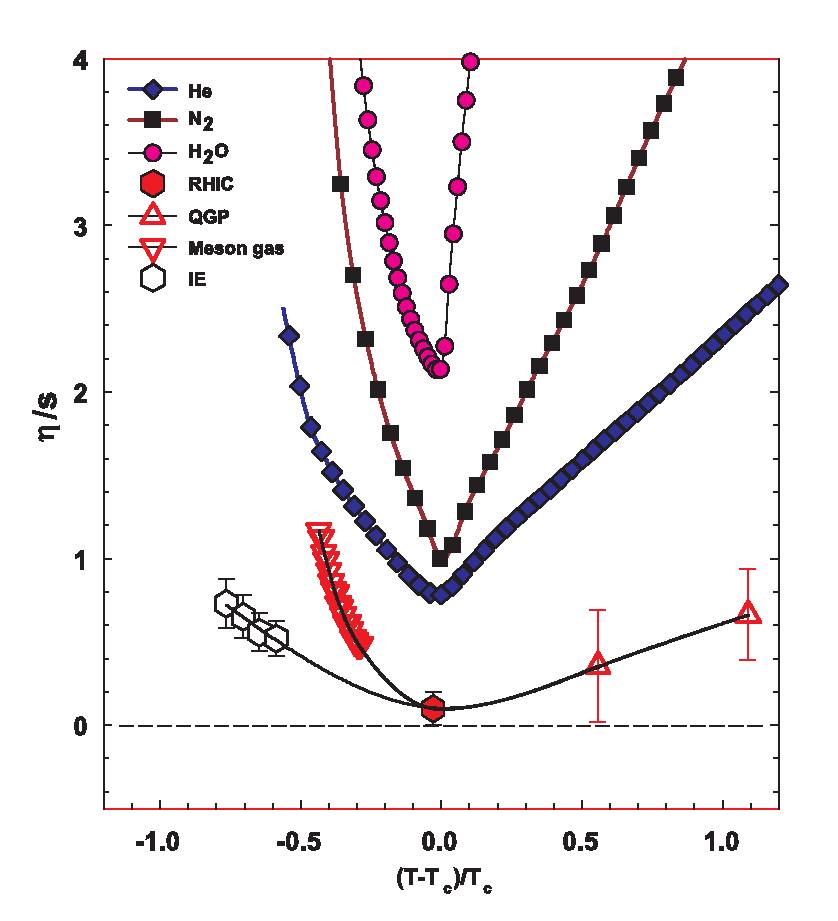
\includegraphics[width=0.5\textwidth]{pics/eta-s-vs-t-tc3}
\caption[$\eta/s$ vs $(T-T_c)/T_c$]{\label{fig3}$\eta/s$ as a function of $(T-T_c)/T_c$ for several substances as indicated. The $\nicefrac{\eta}{s}=0.09\pm0.015$ estimate at RHIC comes from Au-Au collisions at $\sqrt{s_{NN}}=\unit[200]{\gev}$. 
	The calculated values for the meson-gas have an associated error 
	of $\sim$ 50\% %~\cite{Chen:2006ig}. 
	The lattice QCD value $T_c = 170$~MeV %~\cite{Karsch:2000kv} 
	is assumed for nuclear matter. The lines are drawn to guide the eye.~\cite{PhysRevLett.98.092301}
}
\label{fig:etas}
\end{figure}



\FloatBarrier
\pagebreak
\subsection{Heavy-ion physics}
The Quark Gluon Plasma (QGP) is experimentally accessible by colliding heavy-ions at high energies. Nowadays research of Heavy-Ion Collisions is mainly performed at two particle colliders; The Relativistic heavy-ion Collider (RHIC) at BNL in New York, USA and he Large Hadron Collider (LHC) at CERN in Switzerland. Energy densities at these colliders should be enough to produce QGP and convincing evidence of the creation has been seen at both colliders. Complimentary research with heavy nuclei is also performed at the Super Proton Synchrotron (SPS) at CERN.

The development of heavy-ion physics is strongly connected to the development of particle colliders. Experimental study of relativistic heavy-ion collisions has been carried out for three decades, beginning with the Bevalac at Lawrence Berkeley National Laboratory (LBNL)~\cite{Lofgren_1975}, and continuing with the AGS at Brookhaven National Laboratory (BNL)~\cite{Barton:1987}, CERN SPS~\cite{Vitev:2002pf}, RHIC at BNL and LHC at CERN. 

%The first colliders could not produce enough energy to create QGP matter so they could only probe the hadronic state. 
%
%The collective motion of matter in a heavy-ion collision has been modeled using several models e.g. the Blast wave Model~\cite{PhysRevC.84.064905} has been used succesfully. Another model growing in popularity is the hydrodynamical approach which is further discussed in section \ref{sec:hydro}.

\subsubsection{History}
The first heavy-ion collisions were performed at the Bevalac experiment at the Lawrence Berkeley National Laboratory~\cite{Lofgren_1975} and at the Joint Institute for Nuclear Research in Dubna~\cite{kovalenko1994status} at energies up to 1$\gev$ per nucleon.
In 1986 the Super Proton Synchrotron (SPS) at CERN started to look for QGP signatures in O+Pb collisions. The center-of-mass energy per colliding nucleon pair $\left(\sqrt{s_{NN}}\right)$ was \unit[19.4]{GeV}~\cite{Vitev:2002pf}. These experiments did not find any decisive evidence of the existence of QGP. In 1994 a heavier lead (Pb) beam was introduced for new experiments at $\sqrt{s_{NN}}\approx \unit[17]{\gev}$. At the same time the Alternating Gradient Synchrotron (AGS) at BNL, Brookhaven collided ions up to $\mathrm{^{32}S}$ with a fixed target at energies up to \unit[28]{\gev}~\cite{Barton:1987}. In 2000 CERN~\cite{SPSpress} presented compelling evidence for the existence of a new state of matter. Now SPS is used with 400 GeV proton beams for fixed-target experiments, such as the SPS heavy-ion and Neutrino Experiment (SHINE)~\cite{Grebieszkow:2013nza}, which tries to search for the critical point of strongly interacting matter.

The Relativistic heavy-ion Collider (RHIC) at BNL in New York, USA started its  operation in 2000. The top center-of-mass energy per nucleon pair at RHIC, \unit[200]{\gev}, was reached in the following years. The results from the experiments at RHIC have provided a lot of convincing evidences that QGP was created~\cite{Adcox:2004mh, Adams:2005dq, Arsene:2004fa, Back:2004je}. The newest addition to the group of accelerators capable of heavy-ion physics is the Large Hadron Collider (LHC) at CERN, Switzerland. LHC started operating in November 2009 with proton-proton collisions. First Pb-Pb heavy-ion runs started in November 2010 with $\sqrt{s_{NN}}=2.76\; \mathrm{TeV}$,  over ten times higher than at RHIC. Since then LHC has provided both \PbPb and \pPb collisions and a short period of XeXe collisions. Table~\ref{tab:datasets} shows a summary of these. Among the six experiments at LHC, the Large Ion Collider Experiment (ALICE) is dedicated to heavy-ion physics. Also CMS and ATLAS have active heavy-ion programs and LHCb uses its SMOG~\cite{Maurice:2017iom} to perform unique fixed target collisions with heavy ions. 


\begin{table}[htb]
\centering
\caption{Summary of datasets. The integrated luminosities are from ALICE.}
\label{tab:datasets}
\begin{tabular}{| c | S | c |}
\hline
\multicolumn{3}{| c |}{Run 1 (2009-2013)} \\
\hline
\multirow{4}{*}{\pp} & 0.9 \tev & $\sim \unit[200]{\mu b^{-1}}$ \\
 & 2.76 \tev & $\sim \unit[100]{n b^{-1}}$ \\
 & 7.0 \tev & $\sim \unit[1.5]{p b^{-1}}$ \\
 & 8.0 \tev & $\sim \unit[2.5]{p b^{-1}}$ \\
 \hline
\pPb & 5.02 \tev & $\sim\unit[15]{n b^{-1}}$ \\
\hline
\PbPb & 2.76 \tev & $\sim \unit[75]{\mu b^{-1}}$ \\
\hline
\end{tabular}
\begin{tabular}{| c | S | c |}
\hline
\multicolumn{3}{| c |}{Run 2 (2015-2018)} \\
\hline
\multirow{2}{*}{\pp} & 5.02 \tev & $\sim \unit[1.3]{p b^{-1}}$ \\
 & 13.0 \tev & $\sim \unit[25]{p b^{-1}}$ \\
 \hline
\multirow{2}{*}{\pPb} & 5.02 \tev & $\sim\unit[3]{n b^{-1}}$ \\
& 8.16 \tev & $\sim\unit[25]{n b^{-1}}$ \\
\hline
XeXe & 5.44 \tev & $\sim \unit[0.3]{\mu b^{-1}}$ \\
\hline
\PbPb & 5.02 \tev & $\sim \unit[1]{n b^{-1}}$ \\
\hline
\end{tabular}
\end{table}

\pagebreak
\FloatBarrier
%\pagebreak
\subsection{Features of Heavy-Ion Collisions}
\label{sec:features}
\subsubsection{Collision Geometry}
In contrast to protons atomic nuclei are objects with considerable transverse size. The properties of a heavy-ion collision depend strongly on the impact parameter $\vec b$ which is the vector connecting the centres of the two colliding nuclei at their closest approach. One illustration of a heavy-ion collision is shown in Fig.~\ref{fig:planes}.


Impact parameter defines the reaction plane which is the plane spanned by $b$ and the beam direction. $\Psi_{RP}$ gives the angle between the reaction plane and some reference frame angle. Experimentally the reference frame is fixed by the detector setup. Reaction plane angle cannot be directly measured in high energy nuclear collisions, but it can be estimated with the event plane method~\cite{Voloshin:2008dg}. 
\begin{figure}[h!]
\centering
\includegraphics[width=0.6\textwidth]{pics/Definitions}
\caption[The definitions of the Reaction Plane and Participant Plane coordinate systems]{The definitions of the Reaction Plane and Participant Plane coordinate systems~\cite{Voloshin:2007pc}. The dashed circles represent the two colliding nuclei and the green dots are partons that take part  in the collision. $x_{PP}$ and $x_{RP}$ are the participant and reaction planes. The angle between $x_{RP}$ and $x_{PP}$ is given by Eq. (\ref{eq:partangle}). $y_{PP}$ and $y_{RP}$ are lines perpendicular to the participant and reaction planes. }
\label{fig:planes}
\end{figure}


%The constituents in the nucleus have a quantum character and are situated in a potential well. 
%Nucleus density
%This causes fluctuations in the initial geometry of the overlapping region. 
Participant zone is the area containing the participants. The distribution of nucleons in the nucleus exhibits time-dependent fluctuations. Because the nucleon distribution at the time of the collision defines the participant zone, the axis of the participant zone fluctuates and can deviate from the reaction plane. The angle between the participant plane and the reaction plane is defined by ~\cite{Holopainen:2010gz}

\begin{equation}
\psi_{PP}=\arctan \frac{-2\sigma_{xy}}{\sigma_y^2-\sigma_x^2+\sqrt{\left(\sigma_y^2-\sigma_x^2\right)^2+4\sigma_{xy}^2}},
\label{eq:partangle}
\end{equation}

\noindent where the $\sigma$-terms are averaged over the energy density.

\begin{equation}
\sigma_y^2=\langle y^2\rangle-\langle y \rangle ^2, \sigma_x^2=\langle x^2\rangle-\langle x \rangle ^2, \sigma_{xy}=\langle xy \rangle - \langle x \rangle \langle y \rangle
\end{equation}

The impact parameter is one way to quantize the centrality of a heavy-ion collision but it is impossible to measure in a collision. It can be estimated from observed data using theoretical models, but this is always model-dependent and to compare results from different experiments one needs an universal definition for centrality. %The difference between central and peripheral collisions is illustrated in Fig.~\ref{fig:collisionA}. In a central collision the overlap region is larger than in a peripheral collision. Larger overlap region translates into a larger number of nucleons participating in the collision, which in turn leads to a larger number of particles produced in the event.


\begin{figure}[h!]
\centering
        \begin{subfigure}[b]{0.45\textwidth}
                \centering
            	\includegraphics[height=1in]{pics/Collisionperipheral}
                \caption{Peripheral collision}
                \label{fig:peripheral}
        \end{subfigure}
        \begin{subfigure}[b]{0.45\textwidth}
                \centering
               \includegraphics[height=1in]{pics/Collisioncentral}
                \caption{Central collision}
                \label{fig:central}
        \end{subfigure}
        \caption[Interaction between partons in central and peripheral collisions.]{Interaction between partons in central and peripheral collisions. The snowflakes represent elementary parton-parton collisions. When the impact parameter $b$ is large the number of elementary collisions is small. Particle production is small. Smaller impact parameter increases the number of elementary collisions. This increases  particle production.}\label{fig:collisionA}
\end{figure}

Instead in practice centrality is defined by dividing collision events into percentile bins by the number participants or experimentally by the observed multiplicity. Centrality bin 0-5\% corresponds to the most central collisions with the highest multiplicity and higher centrality percentages correspond to more peripheral collisions with lower multiplicities. A multiplicity distribution from ALICE measurements~\cite{PhysRevC.88.044909} illustrating the centrality division is shown in Fig.~\ref{fig:centrality}. The distribution is fitted using a phenomenological approach based on a Glauber Monte Carlo~\cite{Miller:2007ri} plus a convolution of a model for the particle production and a negative binomial distribution. 


\begin{figure}[htb]
\centering

               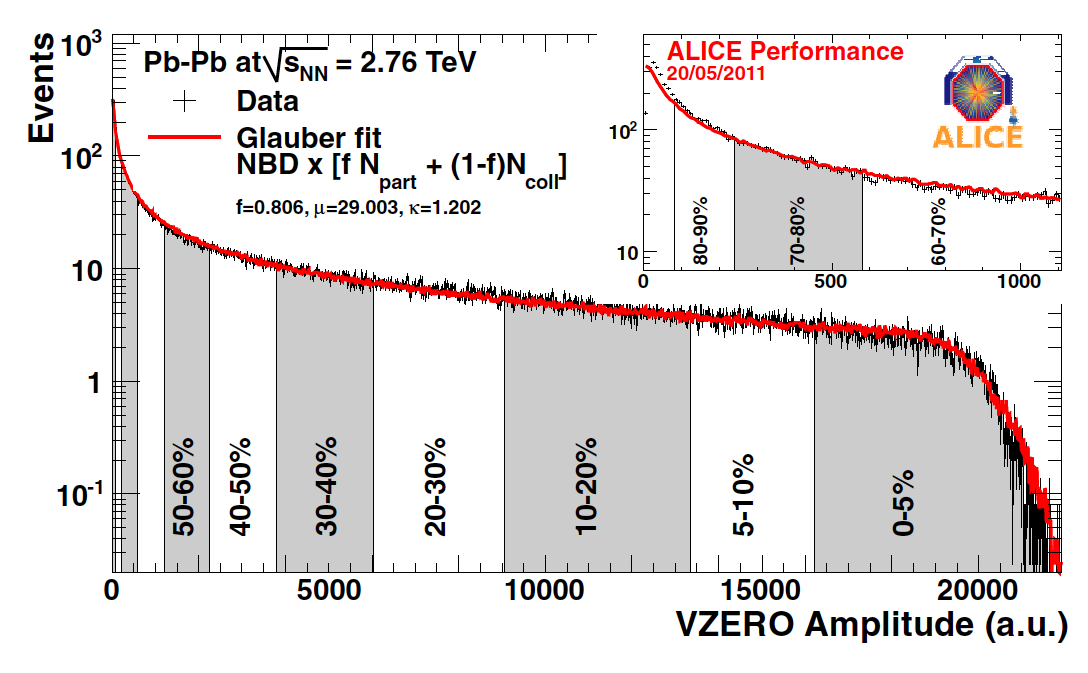
\includegraphics[width=0.9\textwidth]{pics/centrality.png}
        \caption[An illustration of the multiplicity distribution in ALICE measurement with centrality classes.]{An illustration of the multiplicity distribution in ALICE measurements. The red line shows
the fit of the Glauber calculation to the measurement. The data is divided into centrality bins~\cite{PhysRevC.88.044909}. The size of the bins corresponds to the indicated percentile.}
        	\label{fig:centrality}
\end{figure}

%Each centrality bin is obtained by taking the indicated percentile of events arranged by the observed multiplicity. 
%Centrality bin 0-5\% corresponds to the most central collisions. It includes the 5\% of the events  with highest multiplicity. Centralities 90-100\% correspond to the most peripheral collisions. 


%\subsubsection{Nuclear Geometry}
%\label{sec:glauber}
%To model heavy-ion collisions one must first have a description as good as possible of the colliding objects. Atomic nuclei are complex ensembles of nucleons. The nuclei used in heavy-ion physics have in the order of 200 nucleons. Mostly used nuclei are $\mathrm{^{208}Pb}$ at LHC and $\mathrm{^{197}Au}$ at RHIC. The distribution of these nucleons within a nucleus is not uniform and is subject to fluctuations in time.

\subsubsection{Glauber Model}
\label{sec:glauber}
Nuclear geometry in heavy-ion collisions is often modelled with the Glauber Model. The model was originally developed to address the problem of high energy scattering with composite particles. Glauber presented his first collection of papers and unpublished work in his 1958 lectures~\cite{Glauber:1959}. In the 1970's Glauber's work started to have utility in describing total cross sections, after Maximon and Czyz applied it to proton-nucleus and nucleus-nucleus collisions in 1969~\cite{Czyz:1969}. 

In 1976 ~\cite{Biallas1976461} Białłas, Bleszyński, and Czyż applied Glauber's approach to inelastic nuclear collisions. Their approach introduced the basic functions used in modern language including the thickness function and the nuclear overlap function. Thickness function is the integral of the nuclear density over a line going through the nucleus with minimum distance $s$ from its center

\begin{equation}
T_A\left(s\right)=\int_{-\infty}^{\infty}\dd z \rho\left(\sqrt{s^2+z^2}\right).
\end{equation}

\noindent This function gives the thickness of the nucleus, i.e. the amount material seen by a particle passing through it. 

Overlap function is an integral of the thickness functions of two colliding nuclei over the overlap area. This can be seen as the material that takes part in the collision. It is given as a function of the impact parameter $b$

\begin{equation}
T_{AB}\left(\vec b\right)=\int \dd{^2s} T_A\left(\vec s\right) T_B\left(\vec s - \vec b\right)
\end{equation}

\noindent The average overlap function, $\left<T_{AA}\right>$, in an A-A collisions  is given by~\cite{Afanasiev:2009aa}

\begin{equation}
\left<T_{AA}\right>=\frac{\int T_{AA}\left(b\right) \dd b}
{\int\left(1-e^{-\sigma^{inel}_{pp}T_{AA}\left(b\right)}\right)\dd b}.
\end{equation}

\noindent Using $\left<T_{AA}\right>$ one can calculate the mean number of binary collisions

\begin{equation}
\left<N_{coll}\right>=\sigma_{pp}^{inel}\left<T_{AA}\right>,
\end{equation}

\noindent where the total inelastic cross-section, $\sigma_{pp}^{inel}$, gives the probability of two nucleons interacting. The number of binary collisions is related to the hard processes in a heavy-ion collision. Each binary collision has equal probability for direct production of high-momentum partons. Thus the number of high momentum particles is proportional to $\left<N_{coll}\right>$~\cite{Abelev:2013qoq,Kharzeev:2004if,Deng:2010mv}.

Soft production on the other hand is related to the number of participants~\cite{Kharzeev:2004if}. It is assumed that in the binary interactions participants get excited and further interactions are not affected by previous interactions because the time scales are too short for any reaction to happen in the nucleons. After the interactions excited nucleons are transformed into soft particle production. Production does not depend on the number of interactions a nucleon has gone through. The average number of participants, $\left<N_{part}\right>$ can also be calculated from the Glauber model 


\begin{eqnarray}
\left<N_{part}^{AB}\left(b\right)\right>&=&\int \dd{^2s} T_A\left(\bar s\right)\left[1-\left[1-\sigma_{NN}\frac{T_B\left(\bar s - \bar b\right)}{B}\right]^B\right] \nonumber \\
 &+ &\int \dd{^2 s} T_B\left(\bar s\right)\left[1-\left[1-\sigma_{NN}\frac{T_A\left(\bar s - \bar b\right)}{A}\right]^A\right].
\end{eqnarray}

%
%
%
%
%The mean number of binary nucleon collisions can be calculated from the average thickness function 
%
%\begin{equation}
%\left<N_{coll}\right>=\sigma_{pp}^{inel}\left<T_{AA}\right>
%\end{equation}
%
%where $\left<T_{AA}\right>$ is the mean Glauber overlap function for the centrality being analysed 
%
%\begin{equation}
%\left<T_{AA}\right>=\frac{\int T_{AA}\left(b\right)}{\int\left(1-e^{-\sigma^{inel}_{pp}T_{AA}\left(b\right)}\right)db}.
%\end{equation}
%
%
%
%Number of participants is related to the bulk production / soft production. 
%


Glauber calculations require some knowledge of the properties of the nuclei. One requirement is the nucleon density distribution, which can be experimentally determined by studying the nuclear charge distribution in low-energy electron scattering experiments~\cite{Miller:2007ri}.  The nucleon density is usually parametrized by a Woods-Saxon  distribution

%\begin{equation}
%\rho\left(r\right)=\rho_0 \frac{1+w\left(\frac{r}{R}\right)^2}{1+\exp{\left(\frac{r-R}{a}\right)}}
%,\end{equation}
%
\begin{equation}
\rho\left(r\right)=\frac{\rho_0}{1+\exp{\left(\frac{r-R}{a}\right)}}
,\end{equation}

\noindent where $\rho_0$ is the nucleon density in center of the nucleus, $R$ is the nuclear radius and $a$ parametrizes the depth of the skin. The density stays relatively constant as a function of $r$ until around $R$ where it drops to almost 0 within a distance given by $a$.

Another observable required in the calculations is the total inelastic nucleon-nucleon cross-section $\sigma\mathrm{^{NN}_{inel}}$.  This can be measured in proton-proton collisions at different energies.

There are two often used approaches to Glauber calculations. The optical approximation is one way to get simple analytical expressions for the nucleus-nucleus interaction cross-section, the number of interacting  nucleons and the number of nucleon-nucleon collisions. In the optical Glauber it is assumed that during the crossing of the nuclei the nucleons move independently and they will be essentially undeflected.  

With the increase of computational power at hand the Glauber Monte Carlo (GMC) approach has emerged as a method to get a more realistic description of the collisions. In GMC the nucleons are distributed randomly in three-dimensional coordinate system according to the nuclear density distributions~\cite{Abelev:2013qoq}. Also nuclear parameters, like the radius $R$ can be sampled from a distribution. A heavy-ion collision is then treated as a series of independent nucleon-nucleon collisions, where in the simplest model nucleons interact if their distance  in the plane orthogonal to the beam axis, $d$, satisfies

\begin{equation}
d< \sqrt{\sigma\mathrm{^{NN}_{inel}}}
\end{equation}

\noindent The average number of participants and binary collisions can then be determined by simulating many nucleus-nucleus collisions. The results of one GMC Pb-Pb event with impact parameter $b=\unit[9.8]{fm}$ is shown in Fig.~\ref{fig:GMC}

\begin{figure}[htbp]
\centering
               \includegraphics[width=0.5\textwidth]{pics/glauber_eli}
        \caption[The results of one Glauber Monte Carlo simulation.]{The results of one Glauber Monte Carlo simulation. Big circles with black dotted boundaries represent the two colliding nuclei. The participant zone is highlighted with the solid red line.        
        Small red and blue circles represent nucleons. Circles with thick boundaries are participants i.e. they interact with at least one nucleon from the other nucleus. Small circles with dotted boundaries are spectators which do not take part in the collision.}
        	\label{fig:GMC}
\end{figure}



\subsubsection{Hydrodynamical Modelling}
\label{sec:hydro}
The relativistic version of hydrodynamics has been used to model the deconfined phase of a heavy-ion collision with success. Heavy-ion collisions produce many hadrons going into all directions. It is expected that tools from statistical physics would be applicable to this complexity~\cite{Ollitrault:2007du}. The power of relativistic hydrodynamics lies in its simplicity and generality. Hydrodynamics only requires that there is local thermal equilibrium in the system. In order to reach thermal equilibrium the system must be strongly coupled so that the mean free path is shorter than the length scales of interest~\cite{Romatschke:2009im}.

The use of relativistic hydrodynamics in high-energy physics dates back to Landau~\cite{Landau:1953gs} and the 1950's, before QCD was discovered. Back then it was used in proton-proton collisions. Development of hydrodynamics for the use of heavy-ion physics has been active since the 1980's, including Bjorken's study of boost-invariant longitudinal expansion and infinite transverse flow~\cite{PhysRevD.27.140}. Major steps were taken later with the inclusion of finite size and and dynamically generated transverse size~\cite{Baym:1984sr, PhysRevD.34.794}, a part of which was done at the University of Jyväskylä. The role of hydrodynamics in heavy-ion physics was strengthened when QGP was observed to behave like a liquid by RHIC~\cite{Adcox:2004mh}. 

The evolution of a heavy-ion event can be divided into four stages. A schematic representation of the evolution of the collisions is shown in Fig.~\ref{fig:HISpaceTime}. Stage 1 follows immediately the collision. This is known as the pre-equilibrium stage. Hydrodynamic description is not applicable to this regime because thermal equilibrium is not yet reached. The length of this stage is not known but it is assumed to last about $1\ \mathrm{fm}/c$ in proper time $\tau$. 

\begin{figure}[htb]
\centering
               \includegraphics[width=0.5\textwidth]{pics/HISpaceTime2}
        \caption[Schematic representation of a heavy-ion collision]{Schematic representation~\cite{Romatschke:2009im} of a heavy-ion collision as the function of time and longitudinal coordinates $z$ The various stages of the evolution correspond to proper time $\tau=\sqrt{t^2-z^2}$ which is shown as hyperbolic curves separating the different stages.}
        	\label{fig:HISpaceTime}
\end{figure}

The second stage is the regime where thermal equilibrium or at least near-equilibrium is reached. In this stage hydrodynamics should be applicable if the temperature is above the deconfinement temperature~\cite{Romatschke:2009im}. This lasts about $5-10\ \mathrm{fm}/c$ until the temperature of the system sinks low enough for hadronization to occur. Now the system loses its deconfined, strongly coupled, state and hydrodynamics can no longer be used. The third stage is the hadron gas stage where the hadrons still interact. This ends when hadron scattering becomes rare and they no longer interact. In the final stage hadrons are free streaming and they fly in straight lines until they reach the detector.

%The hydrodynamical approach uses. Mass density is not a well defined quantity since pair production and annihilation of quark-antiquark pairs constantly modifies the mass of the system. Instead energy density is used. 

The hydrodynamical approach treats the ensemble of particles as a fluid. It uses  basic equations from hydrodynamics and thermodynamics but with a few modifications to account for the relativistic energies. The calculation is based on a collection of differential equations connecting the local thermal variables like temperature, pressure etc. to local velocities of the fluid. One also needs equations of state that connect the properties of the matter, e.g. temperature and pressure to density.  Given initial conditions and equations of state the calculation gives the time-evolution of the system.

At first only ideal hydrodynamics was used. Ideal hydrodynamics does not include viscosity but it is a relatively good approximation and it could predict phenomena like elliptic flow. For more detailed calculations also viscosity must be considered and viscosity itself is an interesting property of QGP.


\FloatBarrier
\pagebreak
\subsection{Flow}
In a heavy-ion collision the bulk particle production is known as flow. The production is mainly isotropic but a lot of studies including my thesis focus on the small anisotropies. After the formation of the QGP, the matter begins to expand as it is driven outwards by the strong pressure difference between the center of the collision zone and the vacuum outside the collision volume. The pressure-driven expansion is transformed into flow of low-momentum particles in the hadronization phase. Since the expansion is mainly isotropic the resulting particle flow is isotropic with small anisotropic corrections that are of the order of $10\%$ at most. The isotropic part of flow is referred to as radial flow. 

\begin{figure}[b!]
\centering
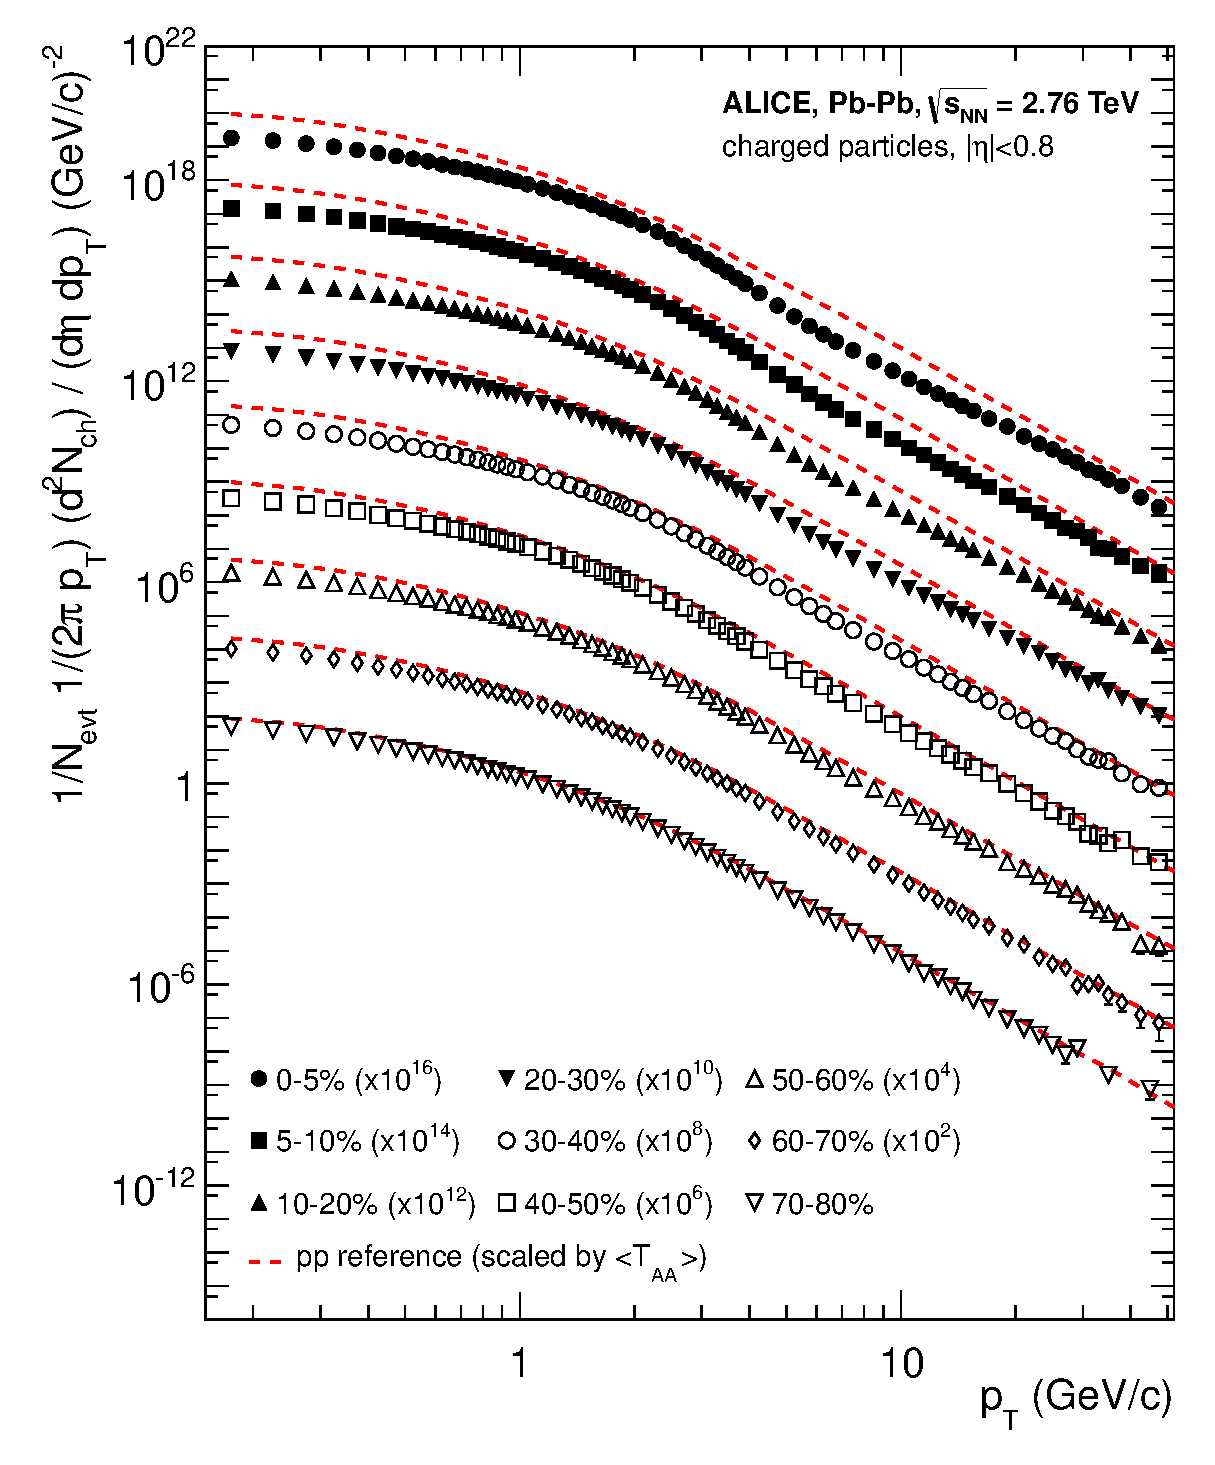
\includegraphics[width=0.6\textwidth]{pics/pT_PbPb}
\caption[Charged particle spectra]{ Charged particle spectra measured by ALICE~\cite{PRL106032301} for the 9 centrality classes given in the legend. The distributions are offset by arbitrary factors given in the legend for clarity. The distributions are offset by arbitrary factors given in the legend for clarity. The dashed lines show the proton-proton reference spectra scaled by the nuclear overlap function determined for each centrality class and by the Pb-Pb spectra scaling factors~\cite{PRL106032301}.}
\label{fig:dndpt}
\end{figure}

The transverse momentum spectra $\dd N/\dd {\pt{}}$ in heavy-ion collisions is shown in Fig. \ref{fig:dndpt}. The vast majority of produced particles have small $\pt{}$. The difference between the yield of $1\gevc$ and $4\gevc$ particles is already 2-3 orders of magnitude. Any observables that are integrated over $\pt{}$ are therefore dominated by the small momentum particles.




\subsubsection{Anisotropic Flow}
In a non-central heavy-ion collision the shape of the impact zone is almond-like. In peripheral collisions the impact parameter is large which means a strongly asymmetric overlap region.  In a central collision the overlap region is almost symmetric in the transverse plane. In this case the impact parameter is small. Collisions with different impact parameters are shown in Fig.~\ref{fig:collisionA}.

\begin{figure}[b!]
\centering
        \begin{subfigure}[b]{0.52\textwidth}
                \centering
            	%\includegraphics[height=2.4in]{pics/InteractionB}
	         \includegraphics[height=2.4in]{figures/tikz/central}

                \caption{Peripheral collision}
                \label{fig:InteractionB}
        \end{subfigure}
        \begin{subfigure}[b]{0.45\textwidth}
                \centering
              % \includegraphics[height=2.4in]{pics/InteractionA}
                \includegraphics[height=2.4in]{figures/tikz/peripheral}

                \caption{Central collision}
                \label{fig:InteractionA}
        \end{subfigure}
	\caption[Illustration of flow in momentum space in central and peripheral collisions.]{Illustration of flow in momentum space in central and peripheral collisions. The density of the arrows represent the magnitude of flow seen at a large distance from the collision in the corresponding azimuthal direction. In a peripheral collision momentum flow into in-plane direction is strong and flow into out-of-plane direction is weak. In a central collision anisotropy in flow is smaller, but the total yield of particles is larger.}
	\label{fig:flow}
\end{figure}

The pressure gradient is largest in-plane, in the direction of the impact parameter $b$, where the distance from high pressure, at the collision center, to low pressure, outside the overlap zone, is smallest. This leads to stronger collective flow into in-plane direction, which in turn results in enhanced thermal emission through a larger effective temperature into this direction, as compared to out-of-plane~\cite{Ollitrault:1992,Ollitrault:1993, Heinz:2002}. The resulting flow is illustrated in Fig.~\ref{fig:flow}. Flow with two maxima in the direction of the reaction plane is called elliptic flow. This is the dominant part of anisotropic flow. Also more complex flow patterns can be identified. The most notable of these is the triangular flow, which is mainly due to fluctuations in the initial conditions.

Flow is nowadays usually quantified in the form of a Fourier composition 

\begin{equation}
E\frac{\dd{^3N}}{\dd {p^3}}=\frac{1}{2\pi}\frac{\dd {^2N}}{\pt{ }\dd {\pt{ }}\dd {\eta} } \left(1+\sum_{n=1}^{\infty}2v_n\left(\pt{},\eta\right)\cos(n(\phi-\Psi_n))\right),
%\label{eq:finalseries}
\end{equation}

\noindent where the coefficients $v_n$ give the relative strengths of different anisotropic flow components and the overall normalisation gives the strength of radial flow. Elliptic flow is represented by $v_2$ and $v_3$ represents triangular flow. The first coefficient, $v_1$, is connected to directed flow. This will however in total be zero because of momentum conservation. It can be nonzero in some rapidity or momentum regions but it must be canceled by other regions.

The first approaches to quantifying the anisotropy of flow did not use the Fourier composition. Instead they approached the problem with a classic event shape analysis using directivity~\cite{danielewicz:1985} or sphericity~\cite{Ollitrault:1992, Danielewicz:1983283} to quantify the flow.


%The first one to predict anisotropic flow in heavy-ion collisions was Ollitrault in 1992~\cite{Ollitrault:1992}. The first papers on anisotropy did not discuss the Fourier composition. Instead they approached the problem with an classic event shape analysis. (sphericity)

The first experimental studies of anisotropy were performed at the AGS~\cite{PhysRevLett.70.1393} in 1993. They noted that the anisotropy of particle production in one region correlates with the reaction plane angle defined in another region. 

The first ones to present the Fourier decomposition were Voloshin and Zhang in 1996~\cite{Voloshin:1994mz}. This new approach was useful for detecting different types of anisotropy in flow, since the different Fourier coefficients give different harmonics in flow. They also show the relative magnitude of each harmonic compared to radial flow.

Some parts of the Fourier composition approach were used for Au-Au collisions at $\snn=11.4\gev$ at AGS in 1994~\cite{Barrette:1994xr}. This analysis still focused on event shapes but they constructed these shapes using Fourier composition from different rapidity windows.


{\color{red} Add a paragraph on the lessions learned from flow studies.}

\FloatBarrier

%\subsubsection{High $\pt{}$ Phenomena}
%The measurement of anisotropic flow coefficients can be extended to very high transverse momenta $\pt{}$. High $\pt{}$ measurements of $v_2$ from CMS~\cite{Chatrchyan:2012xq} are shown in Fig. \ref{fig:highpt}. For high transverse momenta $v_2$ values are positive and they decrease slowly as a function of $\pt{}$. At high transverse momentum the $v_2$ values don't, however, represent flow. 

\FloatBarrier
%\subsubsection{Fluctuations and Event-by-Event Flow}
%The colliding nuclei are not static objects but the distribution of nucleons fluctuates over time. The arrangement of the nucleons at the time of the collision is random, which leads to fluctuations in the initial conditions. The shape of the collision zone is not a perfect almond and it can have a more complex shape. Also the density of the created medium is not homogenous but it can have dense hot spots. The initial density distribution of the created medium is the main reason for anisotropic flow. Because of fluctuations the strength of anisotropic flow is not constant event-by-event.
%
%The existence of more complex density profiles also leads to odd flow harmonics. The basic hydrodynamical approach could only explain elliptic flow and even-harmonics. For a long time it was believed that the odd harmonics would be negligible. In 2007 Mishra {\emph et al.}~\cite{Mishra:2007tw} argued that density inhomogeneities in the initial state would lead to non-zero $v_n$ values for higher harmonics including $v_3$.  It was later noted that higher harmonics of $v_n$ would be suppressed by viscous effects and that the shape of $v_n$ as a function of $n$ would provide another valuable tool for studying $\eta/s$~\cite{Mocsy:2010um}. 
%
%In 2010 significant $v_3$ components were also observed in RHIC data~\cite{Alver:2010gr}. The AMPT model that is also studied in this thesis was able to quantitatively describe the centrality dependence of $v_3$ at RHIC and LHC energies, $\snn=200 \gev$ and $2.76\tev$~\cite{Xu:2011fe}.
%
%%Initial state fluctuations can be modelled using the Glauber model~\cite{Alver:2008zza}. However, so far all models fail to describe the experimental $v_n$ distributions consistently over the whole centrality range~\cite{Jia:2012ve}.
%
%Contrary to elliptic flow higher harmonics are not strongly affected by the centrality of the collision. This supports the theory of higher harmonics being the result of fluctuations. Also $v_2$ measurements of ultra-central collisions give non-zero results for flow, even though the traditional approach based on the anisotropy of the overlap zone gives no prediction of anisotropic flow. This is also the result of fluctuations. Measurement of distributions of $v_n$ coefficients has been performed at ATLAS~\cite{Jia:2012ve}. Their measurements of distributions for $v_2$ in central collisions and for $v_3$ and $v_4$ in general are consistent with a pure Gaussian fluctuation scenario~\cite{Jia:2012ve}.
%
%\begin{figure}[tb]
%	\centering
%	\begin{subfigure}[t]{0.5\textwidth}
%                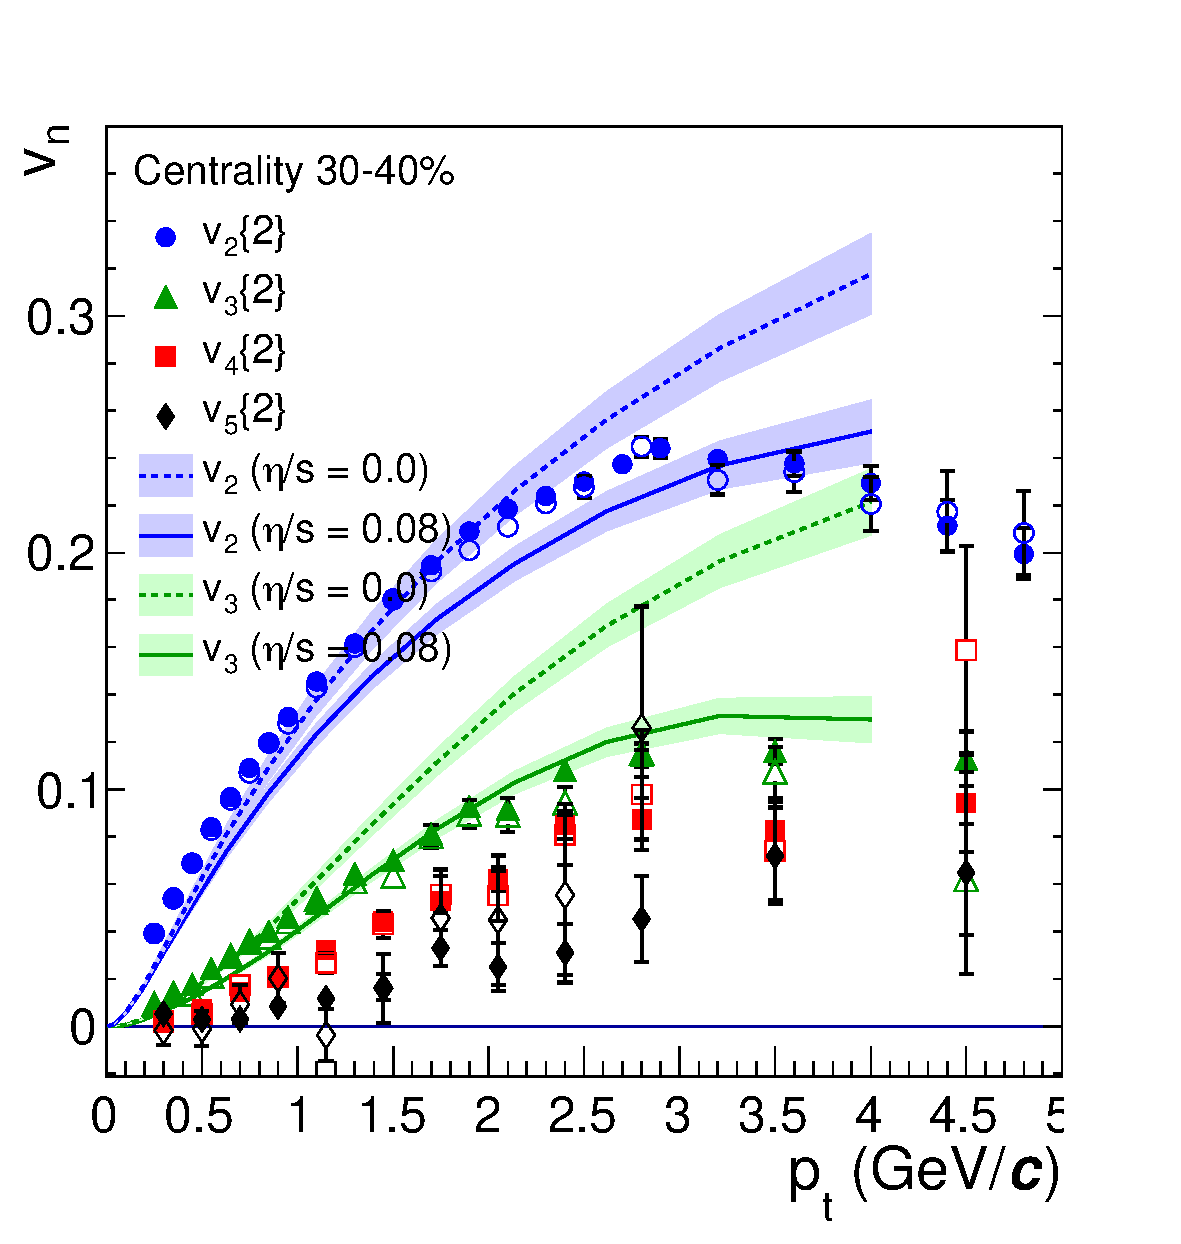
\includegraphics[width=\textwidth]{pics/alice_vn_figa.pdf}
%        \caption[ALICE measurement of $v_2$, $v_3$, $v_4$, $v_5$]{ALICE measurement of $v_2$, $v_3$, $v_4$, $v_5$ as a function of transverse momentum. The flow coefficients are determined by two-particle correlations using different rapidity separations. 
%        The full and open symbols are for $\Delta\eta > 0.2$ and $\Delta\eta > 1.0$. 
%        The results are compared to hydrodynamic predictions~\cite{Schenke:2011tv} with different values of $\eta/s$~\cite{PRL107032301}.}
%        \label{fig:higherharmonics}
%        \end{subfigure}
%        \quad
%        \begin{subfigure}[t]{0.45\textwidth}
%        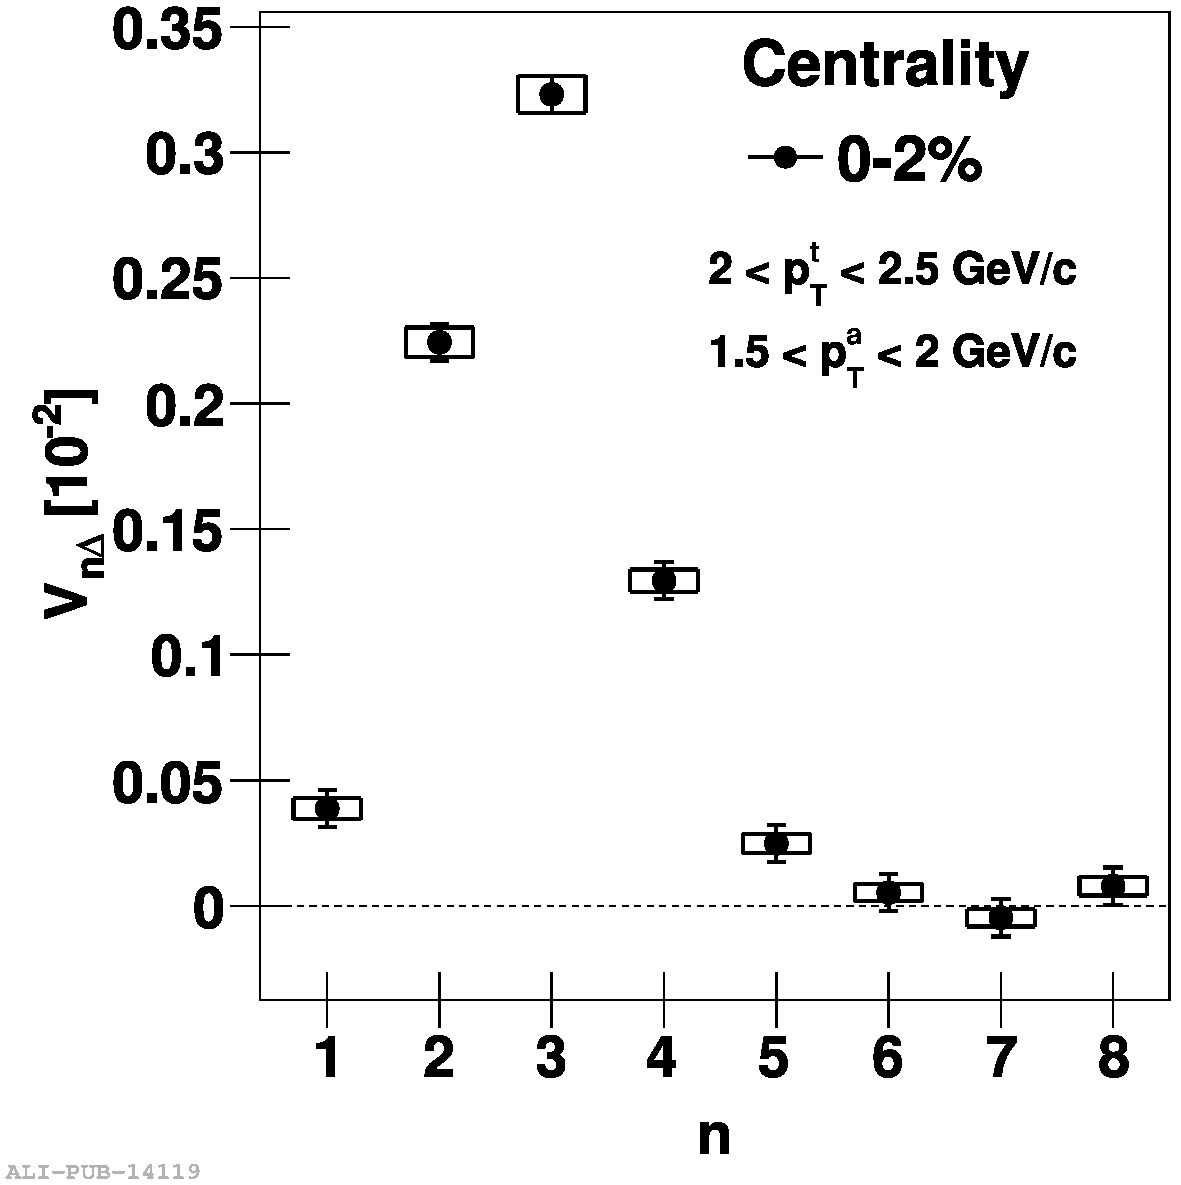
\includegraphics[width=\textwidth]{pics/2012-Jun-06-fig02b}
%        \caption{Amplitude of $v_n$ harmonics as a function of $n$ for the 2\% most central collisions as  measured by ALICE~\cite{Aamodt2012249}.}
%        \label{fig:alicepowers}
%
%        \end{subfigure} 
%        
%%        \begin{subfigure}[t]{\textwidth}
% %               \includegraphics[width=\textwidth]{pics/atlas_powerspectra.png}
%%        \caption{Power spectra of $v_n$ for the 1\% most central collisions measured by ATLAS~\cite{PhysRevC.86.014907}.}
%%        \label{fig:atlaspowers}
% %       \end{subfigure}
%                \caption[Flow measurements of higher harmonics]{Flow measurements of higher harmonics}
%                \label{fig:vnpowers}
%
%\end{figure}
%
%Measurements of different flow harmonics are shown in Fig.~\ref{fig:vnpowers}. The left panel shows different flow harmonics as a function of $\pt{}$ as measured by ALICE~\cite{PRL107032301} in peripheral collisions. In general flow coefficients decrease as a function of $n$ after $n=2$. Central collisions are an exception.The right panel of  Fig.~\ref{fig:vnpowers} shows $v_n$ as a function of $n$ in central collisions as measured by ALICE~\cite{Aamodt2012249}.
%
%
%
%Measurement of event-by-event flow and higher harmonics has growing importance in the field. Triangular flow is useful also for studying jet quenching and in-medium energy loss since anisotropies of flow are related to the path lengths of partons traversing through the medium. Path-lengths and medium density in turn are related the energy loss. An interesting topic of future research would be studying jet properties like $R_{AA}$ separately in events with strong and weak anisotropy.






